\section{genericvcarbiternoflitsNoFlits Class Reference}
\label{classgenericvcarbiternoflitsNoFlits}\index{genericvcarbiternoflitsNoFlits@{genericvcarbiternoflitsNoFlits}}
{\tt \#include $<$genericVcArbiterNoFlits.h$>$}

Inheritance diagram for genericvcarbiternoflitsNoFlits:\nopagebreak
\begin{figure}[H]
\begin{center}
\leavevmode
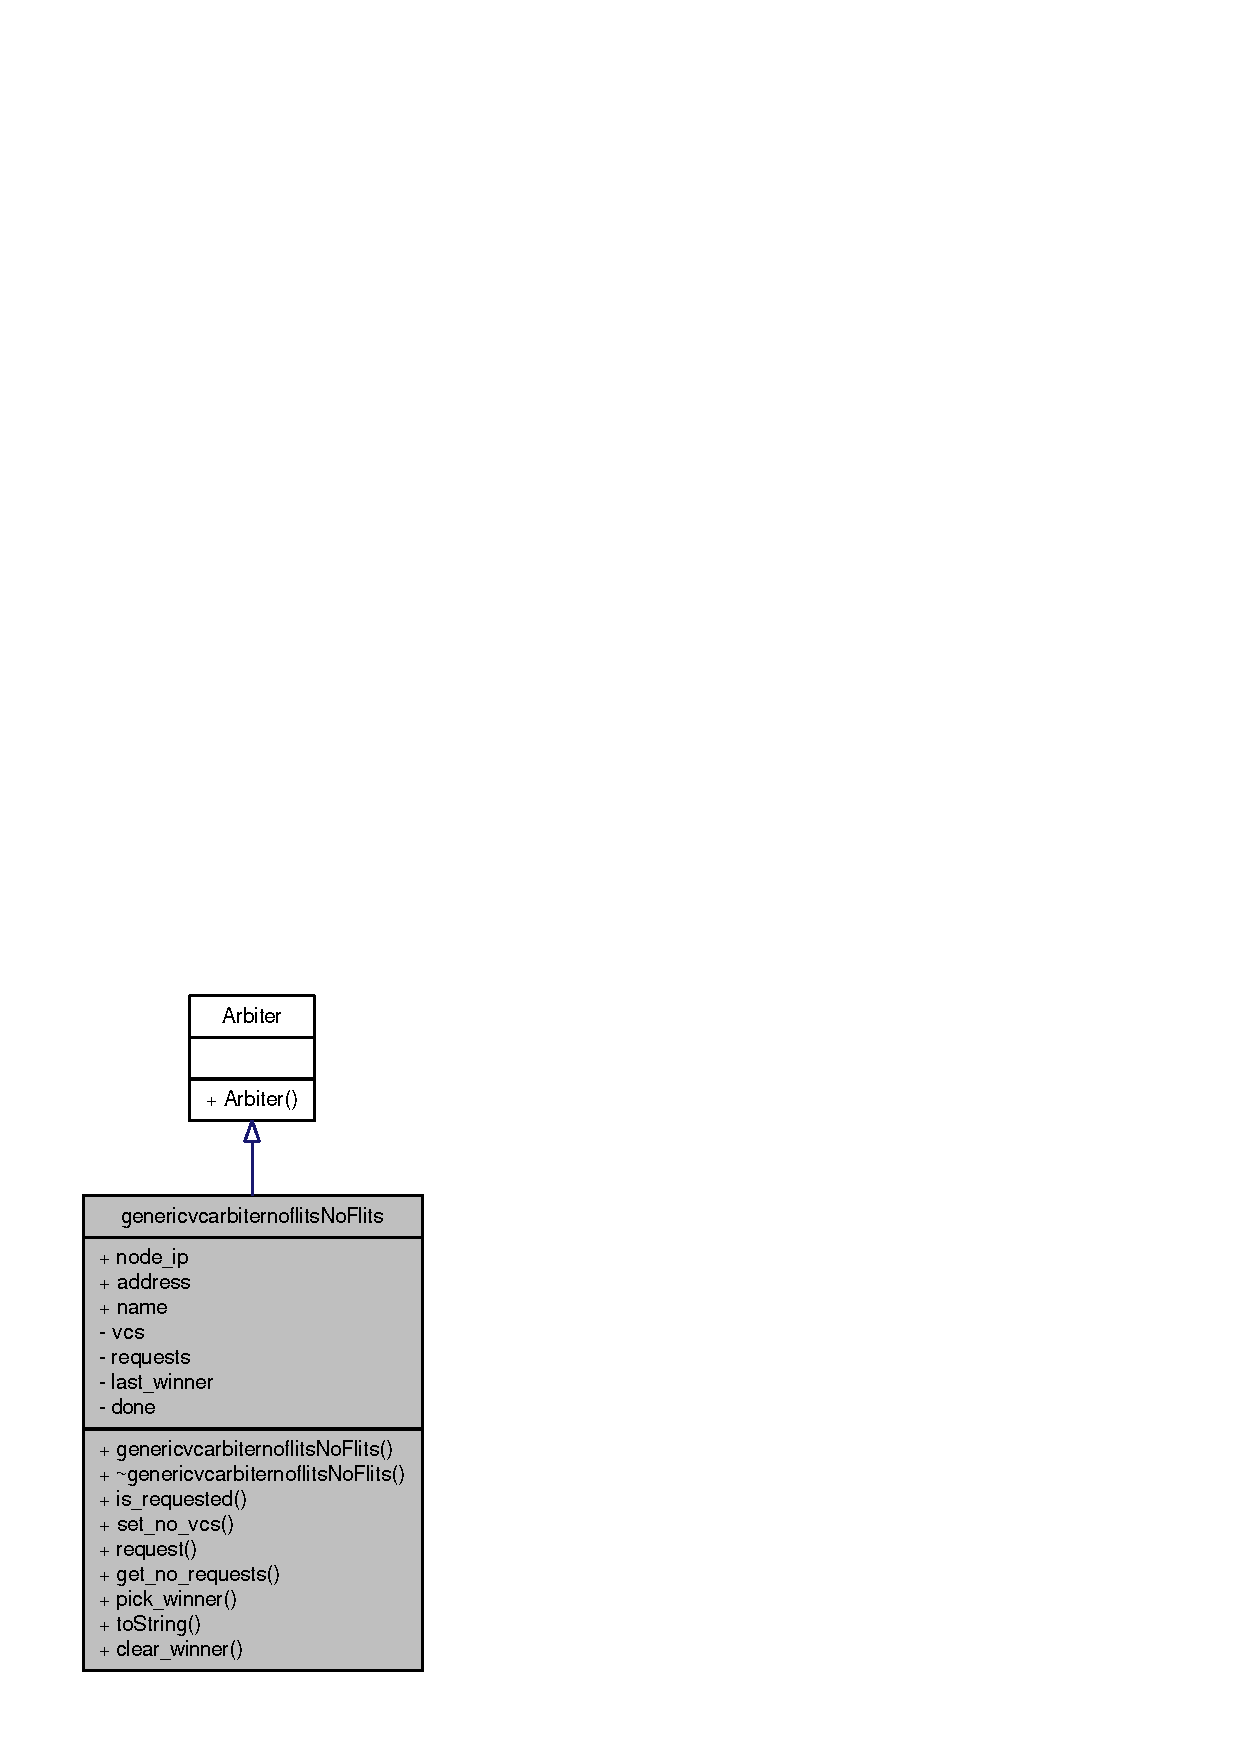
\includegraphics[width=206pt]{classgenericvcarbiternoflitsNoFlits__inherit__graph}
\end{center}
\end{figure}
Collaboration diagram for genericvcarbiternoflitsNoFlits:\nopagebreak
\begin{figure}[H]
\begin{center}
\leavevmode
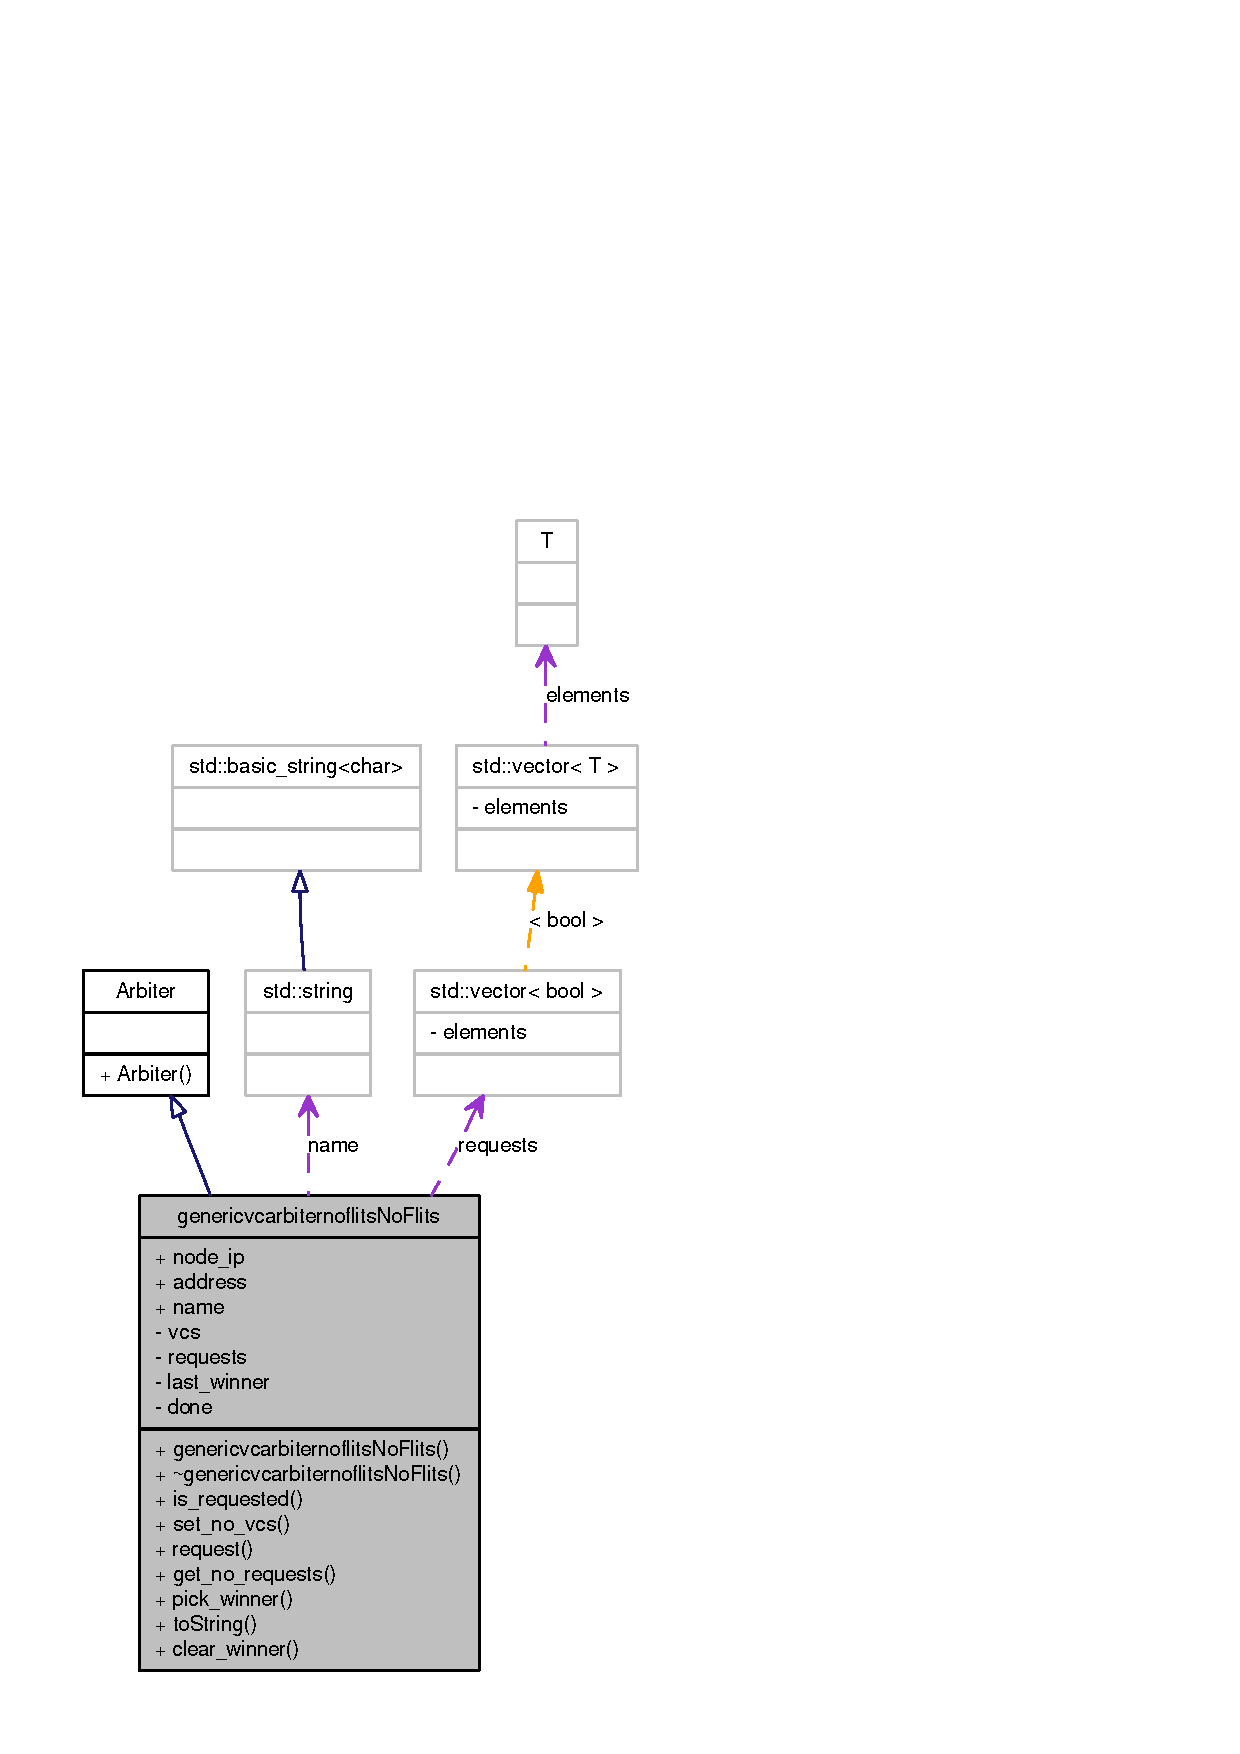
\includegraphics[height=400pt]{classgenericvcarbiternoflitsNoFlits__coll__graph}
\end{center}
\end{figure}
\subsection*{Public Member Functions}
\begin{CompactItemize}
\item 
{\bf genericvcarbiternoflitsNoFlits} ()
\item 
{\bf $\sim$genericvcarbiternoflitsNoFlits} ()
\item 
bool {\bf is\_\-requested} ({\bf uint} ch)
\item 
void {\bf set\_\-no\_\-vcs} ({\bf uint} ch)
\item 
void {\bf request} ({\bf uint} ch)
\item 
{\bf uint} {\bf get\_\-no\_\-requests} ()
\item 
{\bf uint} {\bf pick\_\-winner} ()
\item 
string {\bf toString} () const 
\item 
void {\bf clear\_\-winner} ()
\end{CompactItemize}
\subsection*{Public Attributes}
\begin{CompactItemize}
\item 
{\bf uint} {\bf node\_\-ip}
\item 
{\bf uint} {\bf address}
\item 
string {\bf name}
\end{CompactItemize}
\subsection*{Private Attributes}
\begin{CompactItemize}
\item 
{\bf uint} {\bf vcs}
\item 
vector$<$ bool $>$ {\bf requests}
\item 
{\bf uint} {\bf last\_\-winner}
\item 
bool {\bf done}
\end{CompactItemize}


\subsection{Detailed Description}


Definition at line 31 of file genericVcArbiterNoFlits.h.

\subsection{Constructor \& Destructor Documentation}
\index{genericvcarbiternoflitsNoFlits@{genericvcarbiternoflitsNoFlits}!genericvcarbiternoflitsNoFlits@{genericvcarbiternoflitsNoFlits}}
\index{genericvcarbiternoflitsNoFlits@{genericvcarbiternoflitsNoFlits}!genericvcarbiternoflitsNoFlits@{genericvcarbiternoflitsNoFlits}}
\subsubsection[{genericvcarbiternoflitsNoFlits}]{\setlength{\rightskip}{0pt plus 5cm}genericvcarbiternoflitsNoFlits::genericvcarbiternoflitsNoFlits ()}\label{classgenericvcarbiternoflitsNoFlits_db66d29bba61a5e4bf3ef5ec5d61ce15}




Definition at line 23 of file genericVcArbiterNoFlits.cc.

References address, done, last\_\-winner, name, and node\_\-ip.\index{genericvcarbiternoflitsNoFlits@{genericvcarbiternoflitsNoFlits}!$\sim$genericvcarbiternoflitsNoFlits@{$\sim$genericvcarbiternoflitsNoFlits}}
\index{$\sim$genericvcarbiternoflitsNoFlits@{$\sim$genericvcarbiternoflitsNoFlits}!genericvcarbiternoflitsNoFlits@{genericvcarbiternoflitsNoFlits}}
\subsubsection[{$\sim$genericvcarbiternoflitsNoFlits}]{\setlength{\rightskip}{0pt plus 5cm}genericvcarbiternoflitsNoFlits::$\sim$genericvcarbiternoflitsNoFlits ()}\label{classgenericvcarbiternoflitsNoFlits_337ead5b3dee13995af1c6636f7f3670}




Definition at line 32 of file genericVcArbiterNoFlits.cc.

\subsection{Member Function Documentation}
\index{genericvcarbiternoflitsNoFlits@{genericvcarbiternoflitsNoFlits}!clear\_\-winner@{clear\_\-winner}}
\index{clear\_\-winner@{clear\_\-winner}!genericvcarbiternoflitsNoFlits@{genericvcarbiternoflitsNoFlits}}
\subsubsection[{clear\_\-winner}]{\setlength{\rightskip}{0pt plus 5cm}void genericvcarbiternoflitsNoFlits::clear\_\-winner ()}\label{classgenericvcarbiternoflitsNoFlits_27217b32212845d3c7e3dfe4a87715c4}




Definition at line 73 of file genericVcArbiterNoFlits.cc.

References done, last\_\-winner, and requests.\index{genericvcarbiternoflitsNoFlits@{genericvcarbiternoflitsNoFlits}!get\_\-no\_\-requests@{get\_\-no\_\-requests}}
\index{get\_\-no\_\-requests@{get\_\-no\_\-requests}!genericvcarbiternoflitsNoFlits@{genericvcarbiternoflitsNoFlits}}
\subsubsection[{get\_\-no\_\-requests}]{\setlength{\rightskip}{0pt plus 5cm}{\bf uint} genericvcarbiternoflitsNoFlits::get\_\-no\_\-requests ()}\label{classgenericvcarbiternoflitsNoFlits_21ef6c560a4408fb9233416f384ec434}




Definition at line 62 of file genericVcArbiterNoFlits.cc.

References requests, and vcs.\index{genericvcarbiternoflitsNoFlits@{genericvcarbiternoflitsNoFlits}!is\_\-requested@{is\_\-requested}}
\index{is\_\-requested@{is\_\-requested}!genericvcarbiternoflitsNoFlits@{genericvcarbiternoflitsNoFlits}}
\subsubsection[{is\_\-requested}]{\setlength{\rightskip}{0pt plus 5cm}bool genericvcarbiternoflitsNoFlits::is\_\-requested ({\bf uint} {\em ch})}\label{classgenericvcarbiternoflitsNoFlits_9a0299945d0e4d627534ffcfd06a8921}




Definition at line 55 of file genericVcArbiterNoFlits.cc.

References requests.\index{genericvcarbiternoflitsNoFlits@{genericvcarbiternoflitsNoFlits}!pick\_\-winner@{pick\_\-winner}}
\index{pick\_\-winner@{pick\_\-winner}!genericvcarbiternoflitsNoFlits@{genericvcarbiternoflitsNoFlits}}
\subsubsection[{pick\_\-winner}]{\setlength{\rightskip}{0pt plus 5cm}{\bf uint} genericvcarbiternoflitsNoFlits::pick\_\-winner (void)}\label{classgenericvcarbiternoflitsNoFlits_8d28e69dbcb2e4bd1bce785ade0b4573}




Definition at line 81 of file genericVcArbiterNoFlits.cc.

References done, last\_\-winner, and requests.\index{genericvcarbiternoflitsNoFlits@{genericvcarbiternoflitsNoFlits}!request@{request}}
\index{request@{request}!genericvcarbiternoflitsNoFlits@{genericvcarbiternoflitsNoFlits}}
\subsubsection[{request}]{\setlength{\rightskip}{0pt plus 5cm}void genericvcarbiternoflitsNoFlits::request ({\bf uint} {\em ch})}\label{classgenericvcarbiternoflitsNoFlits_679b8b6bc3be8c5e28635939a10ee2b7}




Definition at line 47 of file genericVcArbiterNoFlits.cc.

References done, and requests.\index{genericvcarbiternoflitsNoFlits@{genericvcarbiternoflitsNoFlits}!set\_\-no\_\-vcs@{set\_\-no\_\-vcs}}
\index{set\_\-no\_\-vcs@{set\_\-no\_\-vcs}!genericvcarbiternoflitsNoFlits@{genericvcarbiternoflitsNoFlits}}
\subsubsection[{set\_\-no\_\-vcs}]{\setlength{\rightskip}{0pt plus 5cm}void genericvcarbiternoflitsNoFlits::set\_\-no\_\-vcs ({\bf uint} {\em ch})}\label{classgenericvcarbiternoflitsNoFlits_6d61b38c12a4dcae8137849232106541}




Definition at line 38 of file genericVcArbiterNoFlits.cc.

References requests, and vcs.\index{genericvcarbiternoflitsNoFlits@{genericvcarbiternoflitsNoFlits}!toString@{toString}}
\index{toString@{toString}!genericvcarbiternoflitsNoFlits@{genericvcarbiternoflitsNoFlits}}
\subsubsection[{toString}]{\setlength{\rightskip}{0pt plus 5cm}string genericvcarbiternoflitsNoFlits::toString () const}\label{classgenericvcarbiternoflitsNoFlits_0cbe88bbc52325a3f4301bcca576e2ea}




Definition at line 109 of file genericVcArbiterNoFlits.cc.

References last\_\-winner, and requests.

\subsection{Member Data Documentation}
\index{genericvcarbiternoflitsNoFlits@{genericvcarbiternoflitsNoFlits}!address@{address}}
\index{address@{address}!genericvcarbiternoflitsNoFlits@{genericvcarbiternoflitsNoFlits}}
\subsubsection[{address}]{\setlength{\rightskip}{0pt plus 5cm}{\bf uint} {\bf genericvcarbiternoflitsNoFlits::address}}\label{classgenericvcarbiternoflitsNoFlits_5160d84b65185cfc3d7942ebb186982c}




Definition at line 37 of file genericVcArbiterNoFlits.h.

Referenced by genericvcarbiternoflitsNoFlits().\index{genericvcarbiternoflitsNoFlits@{genericvcarbiternoflitsNoFlits}!done@{done}}
\index{done@{done}!genericvcarbiternoflitsNoFlits@{genericvcarbiternoflitsNoFlits}}
\subsubsection[{done}]{\setlength{\rightskip}{0pt plus 5cm}bool {\bf genericvcarbiternoflitsNoFlits::done}\hspace{0.3cm}{\tt  [private]}}\label{classgenericvcarbiternoflitsNoFlits_27235d72b4988b915f86484bf9d9f129}




Definition at line 53 of file genericVcArbiterNoFlits.h.

Referenced by clear\_\-winner(), genericvcarbiternoflitsNoFlits(), pick\_\-winner(), and request().\index{genericvcarbiternoflitsNoFlits@{genericvcarbiternoflitsNoFlits}!last\_\-winner@{last\_\-winner}}
\index{last\_\-winner@{last\_\-winner}!genericvcarbiternoflitsNoFlits@{genericvcarbiternoflitsNoFlits}}
\subsubsection[{last\_\-winner}]{\setlength{\rightskip}{0pt plus 5cm}{\bf uint} {\bf genericvcarbiternoflitsNoFlits::last\_\-winner}\hspace{0.3cm}{\tt  [private]}}\label{classgenericvcarbiternoflitsNoFlits_b0be12b7ac81e3a22098252a6bc44bc0}




Definition at line 52 of file genericVcArbiterNoFlits.h.

Referenced by clear\_\-winner(), genericvcarbiternoflitsNoFlits(), pick\_\-winner(), and toString().\index{genericvcarbiternoflitsNoFlits@{genericvcarbiternoflitsNoFlits}!name@{name}}
\index{name@{name}!genericvcarbiternoflitsNoFlits@{genericvcarbiternoflitsNoFlits}}
\subsubsection[{name}]{\setlength{\rightskip}{0pt plus 5cm}string {\bf genericvcarbiternoflitsNoFlits::name}}\label{classgenericvcarbiternoflitsNoFlits_9f7e29c9d9d8568b3178082ed6c76f4e}




Definition at line 38 of file genericVcArbiterNoFlits.h.

Referenced by genericvcarbiternoflitsNoFlits().\index{genericvcarbiternoflitsNoFlits@{genericvcarbiternoflitsNoFlits}!node\_\-ip@{node\_\-ip}}
\index{node\_\-ip@{node\_\-ip}!genericvcarbiternoflitsNoFlits@{genericvcarbiternoflitsNoFlits}}
\subsubsection[{node\_\-ip}]{\setlength{\rightskip}{0pt plus 5cm}{\bf uint} {\bf genericvcarbiternoflitsNoFlits::node\_\-ip}}\label{classgenericvcarbiternoflitsNoFlits_17c531b8bb9df1098347bdfdf50f8bc9}




Definition at line 36 of file genericVcArbiterNoFlits.h.

Referenced by genericvcarbiternoflitsNoFlits().\index{genericvcarbiternoflitsNoFlits@{genericvcarbiternoflitsNoFlits}!requests@{requests}}
\index{requests@{requests}!genericvcarbiternoflitsNoFlits@{genericvcarbiternoflitsNoFlits}}
\subsubsection[{requests}]{\setlength{\rightskip}{0pt plus 5cm}vector$<$ bool $>$ {\bf genericvcarbiternoflitsNoFlits::requests}\hspace{0.3cm}{\tt  [private]}}\label{classgenericvcarbiternoflitsNoFlits_44f82d31aa430702968d2f78d2faca14}




Definition at line 51 of file genericVcArbiterNoFlits.h.

Referenced by clear\_\-winner(), get\_\-no\_\-requests(), is\_\-requested(), pick\_\-winner(), request(), set\_\-no\_\-vcs(), and toString().\index{genericvcarbiternoflitsNoFlits@{genericvcarbiternoflitsNoFlits}!vcs@{vcs}}
\index{vcs@{vcs}!genericvcarbiternoflitsNoFlits@{genericvcarbiternoflitsNoFlits}}
\subsubsection[{vcs}]{\setlength{\rightskip}{0pt plus 5cm}{\bf uint} {\bf genericvcarbiternoflitsNoFlits::vcs}\hspace{0.3cm}{\tt  [private]}}\label{classgenericvcarbiternoflitsNoFlits_773952bc5d23a4b91dcfb3450bfae84d}




Definition at line 50 of file genericVcArbiterNoFlits.h.

Referenced by get\_\-no\_\-requests(), and set\_\-no\_\-vcs().

The documentation for this class was generated from the following files:\begin{CompactItemize}
\item 
{\bf genericVcArbiterNoFlits.h}\item 
{\bf genericVcArbiterNoFlits.cc}\end{CompactItemize}
